\documentclass[12pt,letterpaper]{article}

\usepackage[utf8]{inputenc}
\usepackage[T1]{fontenc}
\usepackage{amsmath}
\usepackage{amsfonts}
\usepackage{amssymb}
\usepackage{amsthm}
\usepackage[left=2cm,right=2cm,top=2cm,bottom=2cm,headheight=22pt]{geometry}
\usepackage{fancyhdr}
\usepackage{setspace}
\usepackage{lastpage}
\usepackage{graphicx}
\usepackage{caption}
\usepackage{subcaption}
\usepackage{paralist}
\usepackage{url}
\usepackage{tikz}

\theoremstyle{definition}
\newtheorem{question}{Question}
\newtheorem{example}{Example}
\newtheorem{exercise}[question]{Exercise}
\newtheorem*{challenge}{Challenge}

\begin{document}

%Paramètres de mise en forme des paragraphes selon les normes françaises
\setlength{\parskip}{1ex plus 0.5ex minus 0.2ex}
\setlength{\parindent}{0pt}

%Paramètres relatifs aux en-têtes et pieds de page.
\pagestyle{fancy}
\lhead{Theron J Hitchman}
\chead{\Large Reading and Guided Practice \#9}
\rhead{Spring 2014}
\lfoot{\emph{Math and Decision Making}}
\cfoot{}
\rfoot{\emph{\thepage\ of \pageref{LastPage}}}

\section*{Introduction}
We see how Reidemeister moves help us to understand that tricolorability is an \emph{invariant} for knots and links. We use this information to finally distinguish two of our favorite examples as different.

\section*{Goals}
At the end of this assignment, a student should be able to:
\begin{compactitem}
\item Discuss what an invariant is.
\item Show how tricolorability is preserved by Reidemeister moves.
\item Explain why tricolorability is a property of a knot or link, and not just a property of a particular diagram.
\end{compactitem}


\section*{Reading and Questions for Topology Meeting 10}

How do we tell two knots apart?
We have a way of saying that two knots are equivalent---we find a sequence of Reidemeister Moves that transforms a planar projection of one knot into a planar projection of the other.
But how do we decide that two  knots or links are definitely \underline{not} equivalent?
Reidemeister moves are helpful, but how do we know we have tried enough of them?
Maybe you have tried all sequences of $1,000,000$ Reidemeister moves or less, but the knots still look different.
That sounds like a big number, so maybe the knots are different.
But it is possible that the shortest number of Reidemeister moves between two knots is $1,000,100$ moves long!
This could happen with a really complicated planar projection.
(Think of a Jackson Pollock painting.)

\subsection*{The Idea of an Invariant}

What we need is something we can measure or compute about a knot or link that helps us tell them apart. And it will be important that this thing is the same for different planar projections of the same knot or link.

This kind of thing is called an \emph{invariant}.
Invariants come in many types: some are numbers, some are answers to yes or no questions, some are more complicated objects. Our object is to introduce an invariant of knots and links of the "yes or no" variety called \emph{tricolorability}.
We have already discussed the idea of tricolorability for a particular planar projection diagram of a knot or link. 
The point of this reading is to see that tricolorability is a property of the knot (or link) and not just of a particular projection.

The main reason for this is the following fact:
\begin{quote}
If one planar projection diagram of a knot (or link) is tricolorable, then so is \emph{any other} planar projection diagram of that knot or link. 
All planar projections of a particular knot are either all tricolorable together, or all not tricolorable together.
\end{quote}

\clearpage

\subsection*{Tricolorability of Related Diagrams}

In the last Reading and Guided Practice, you showed that a projection of the trefoil knot is tricolorable.
Here is a projection of the trefoil with a tricoloring.

\begin{figure}[h]
    \centering
    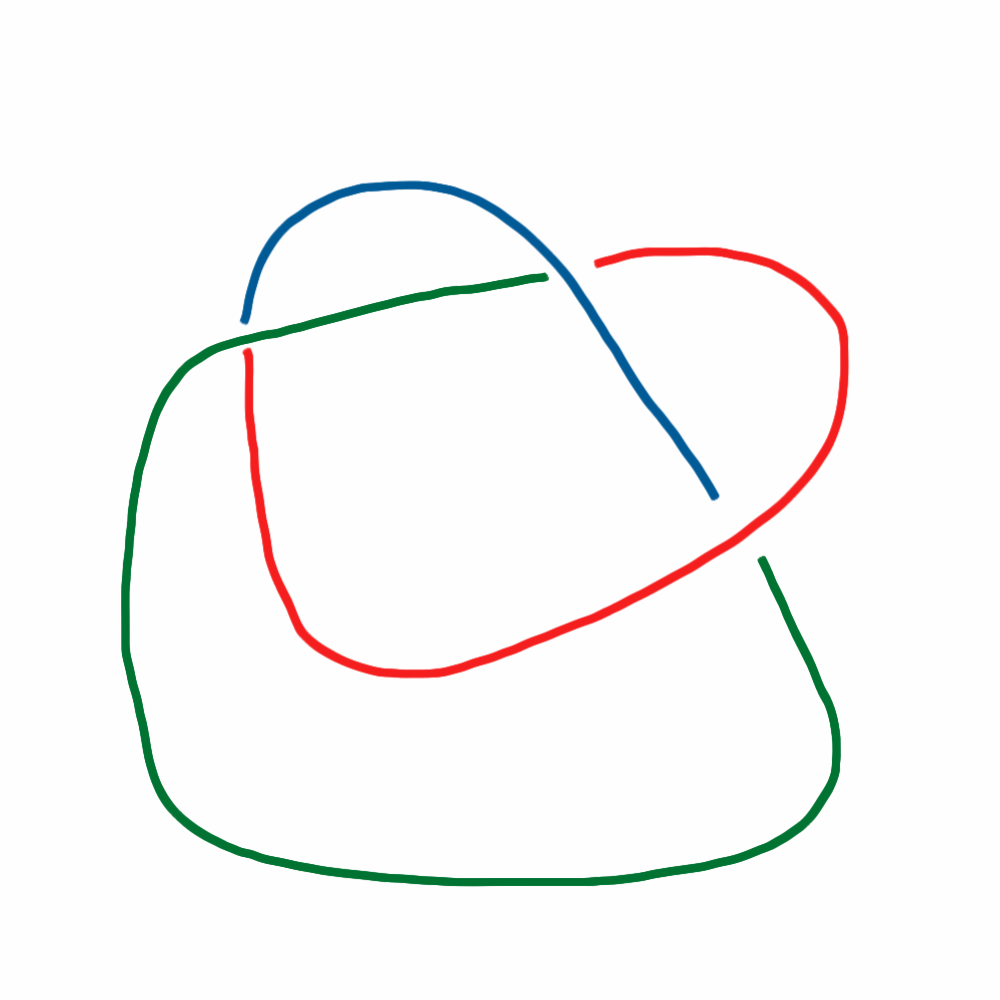
\includegraphics[width=.4\textwidth]{knotpics/tricolor_trefoil.png}
    \caption{A tricoloring of this trefoil projection.}
\end{figure}

\begin{exercise}
Find a way to adjust the coloring scheme from the tricoloring above to show that each of these projections of the trefoil are also tricolorable.
The goal is to change the coloring scheme as little as possible, so 
The parts of the knot that have not moved are colored just like in the original.
Your job is to find the right colors for the black strands.
\end{exercise}

\begin{figure}[h] 
    \centering
    \begin{subfigure}{.3\textwidth}
        \centering
        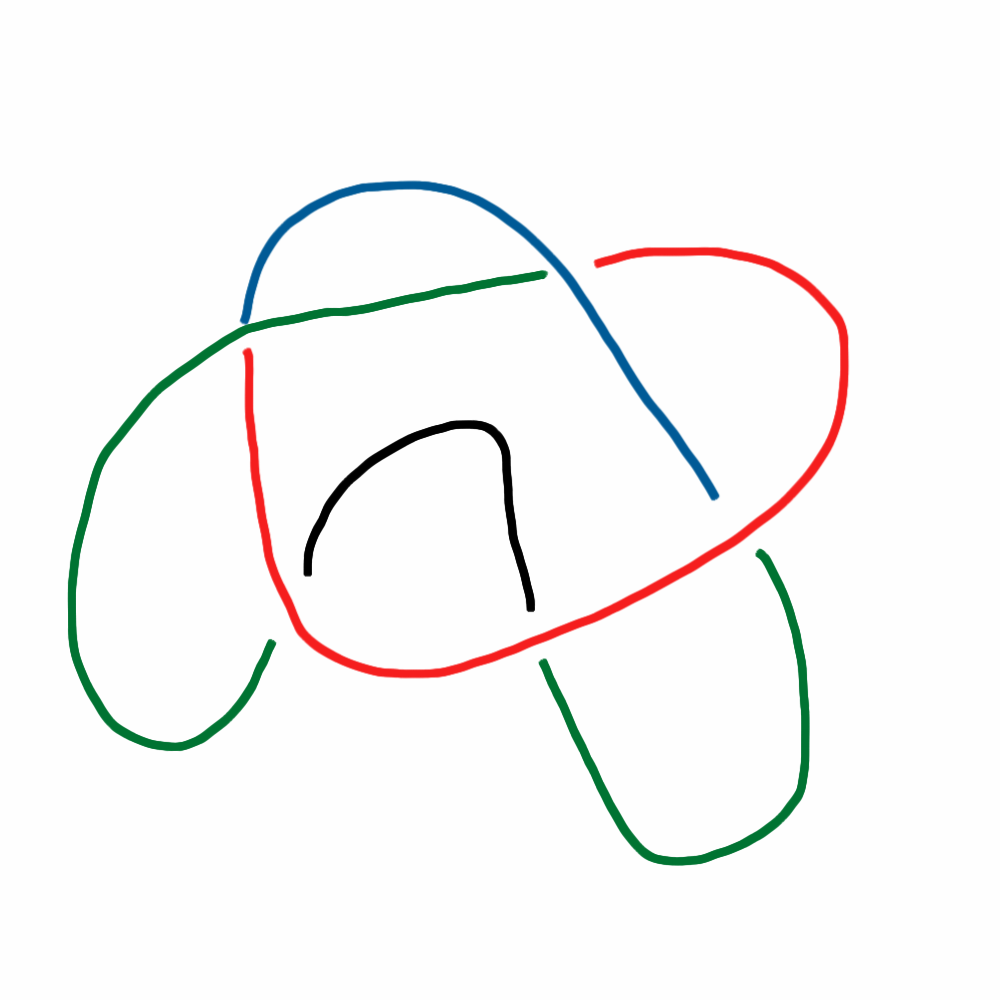
\includegraphics[width=\textwidth]{knotpics/tricolor2.png}
    \end{subfigure}
    \quad
    \begin{subfigure}{.3\textwidth}
        \centering
        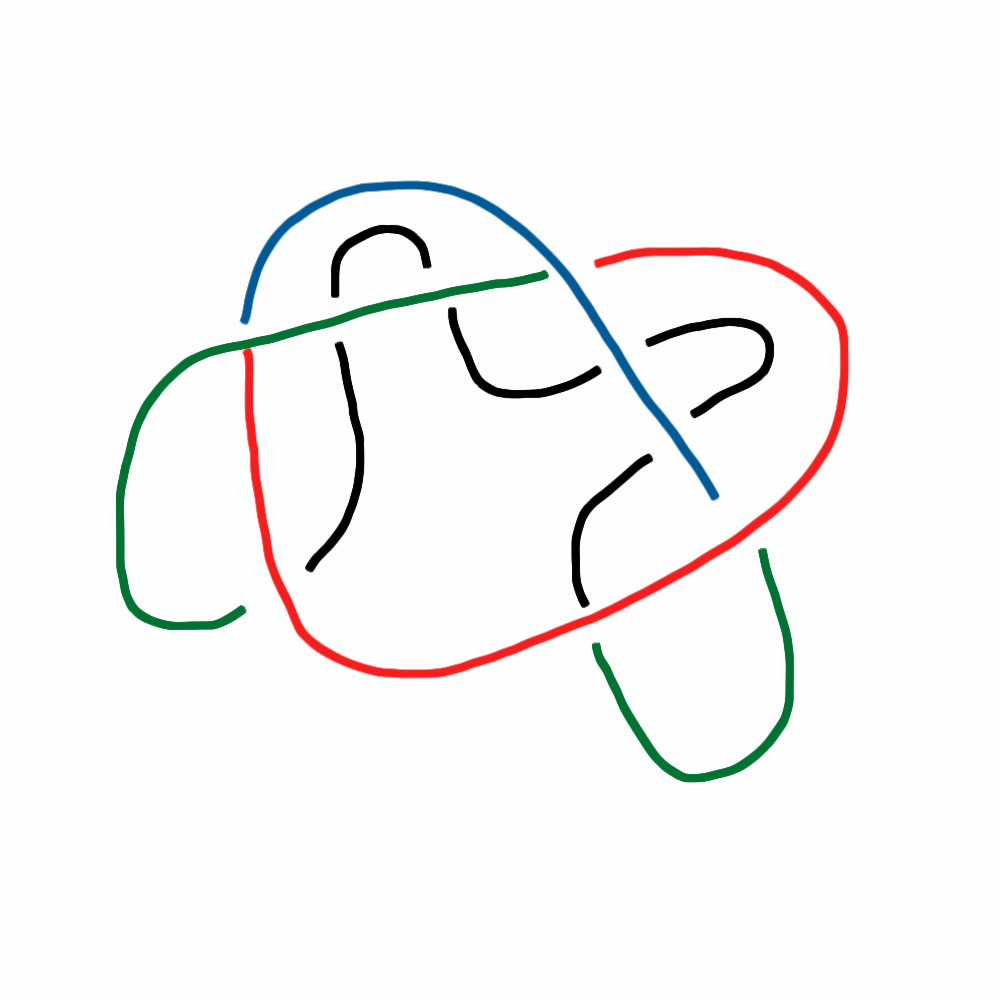
\includegraphics[width=\textwidth]{knotpics/tricolor3.png}
    \end{subfigure}
    \quad
    \begin{subfigure}{.3\textwidth}
        \centering
        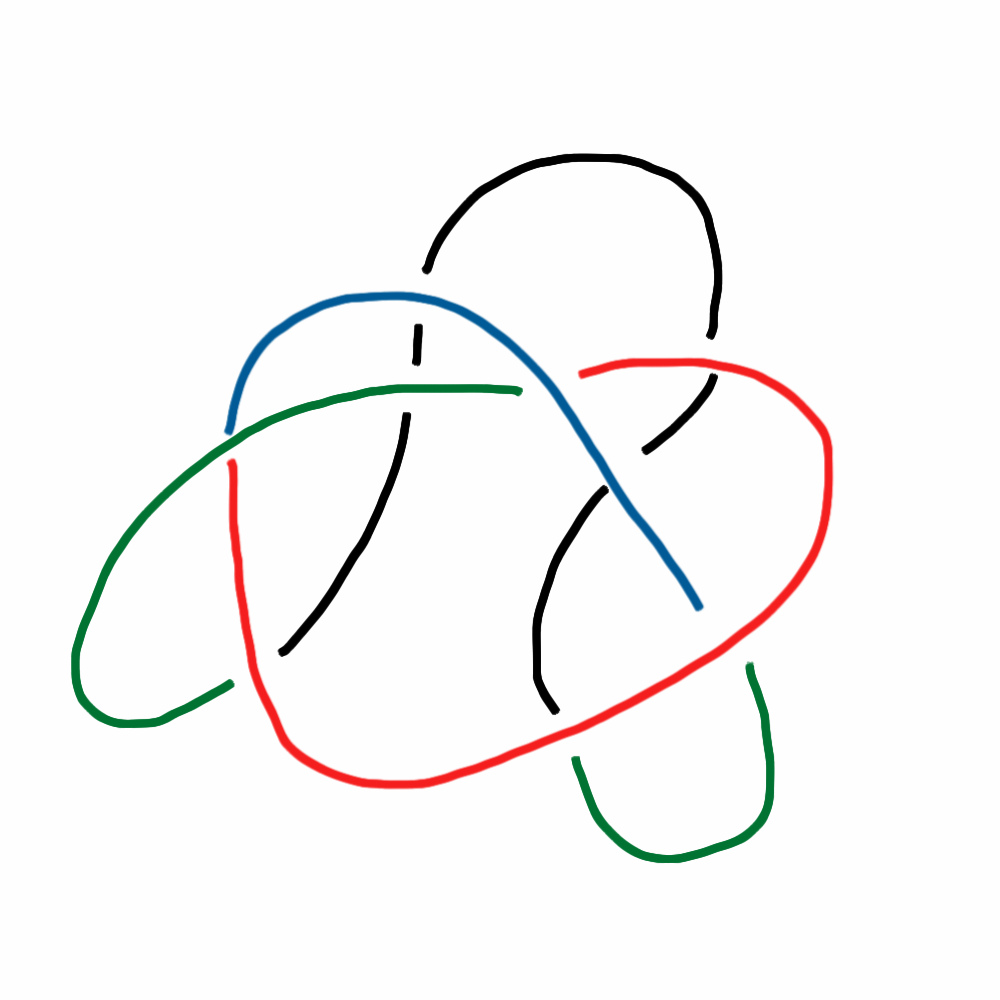
\includegraphics[width=\textwidth]{knotpics/tricolor4.png}
    \end{subfigure}
    \caption{Three more projections of the trefoil.}
\end{figure}


Note that each diagram differs from the previous one by either one or two Reidemeister moves. 
This is the key idea!

\subsection*{Tricolorability is an Invariant}

How do we know that tricolorability is a useful thing?
The key is that performing a Reidemeister move \emph{doesn't change the notion of tricolorability.}
If one planar projection of a knot or link is tricolorable, then performing a Reidemeister move gives us a new planar projection which is also tricolorable.
Similarly, if a planar projection of a knot or link is not tricolorable, then performing a Reidemeister move gives us a new planar projection which is still not tricolorable.
This means that tricolorability is an invariant of knots and links.

How do we see that all of this works as claimed?
We just check the three types of moves with different types of colorings that can happen.
This is a very short list, so it is not difficult to check.

Let us check through some of the Reidemeister moves.
First consider a move of type one.
This only involves a single strand.

\begin{figure}[h]
    \centering
    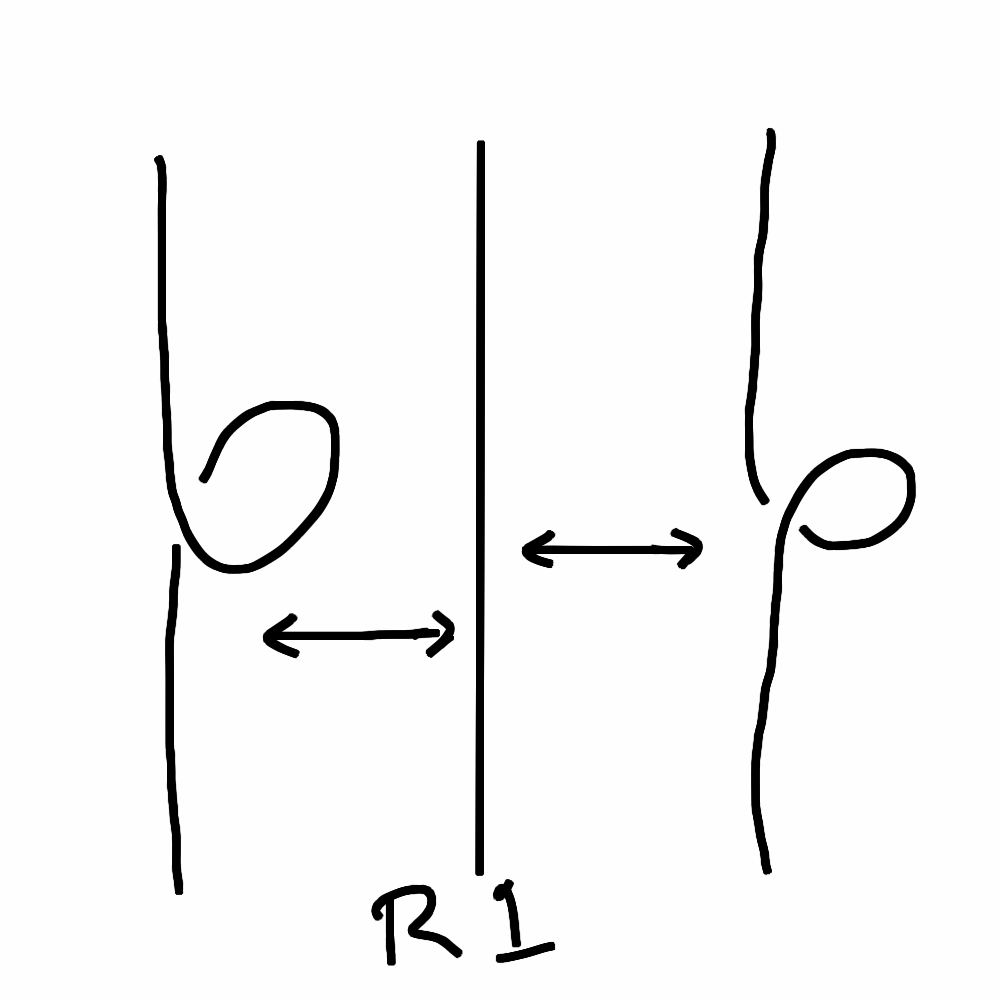
\includegraphics[width=.3\textwidth]{knotpics/r1.png}
    \caption{Reidemeister moves of type one.}
\end{figure}

If we are adding a twist, then the starting strand has only one color.
After we add a twist, leave everything involved that same color.
At the new crossing, all three strands are that color, which fits our rule.
If we are removing a twist, what happens?
First note that a single strand looped over itself must have only one color. This is because at the crossing, one of the understrands comes back around to be the overstrand at the same crossing.
Tricolorability requires that each crossing has either one color or three involved.
We can't have three colors because two of the strands are really the same, so everything in the picture must be a single color.
After removing the twist, just leave the new strand that same color.
Happy and nice.


What about a type two Reidemeister move?
I'll draw the relevant pictures here, and leave you to work out the discussion.

\begin{figure}[h!]
    \centering
    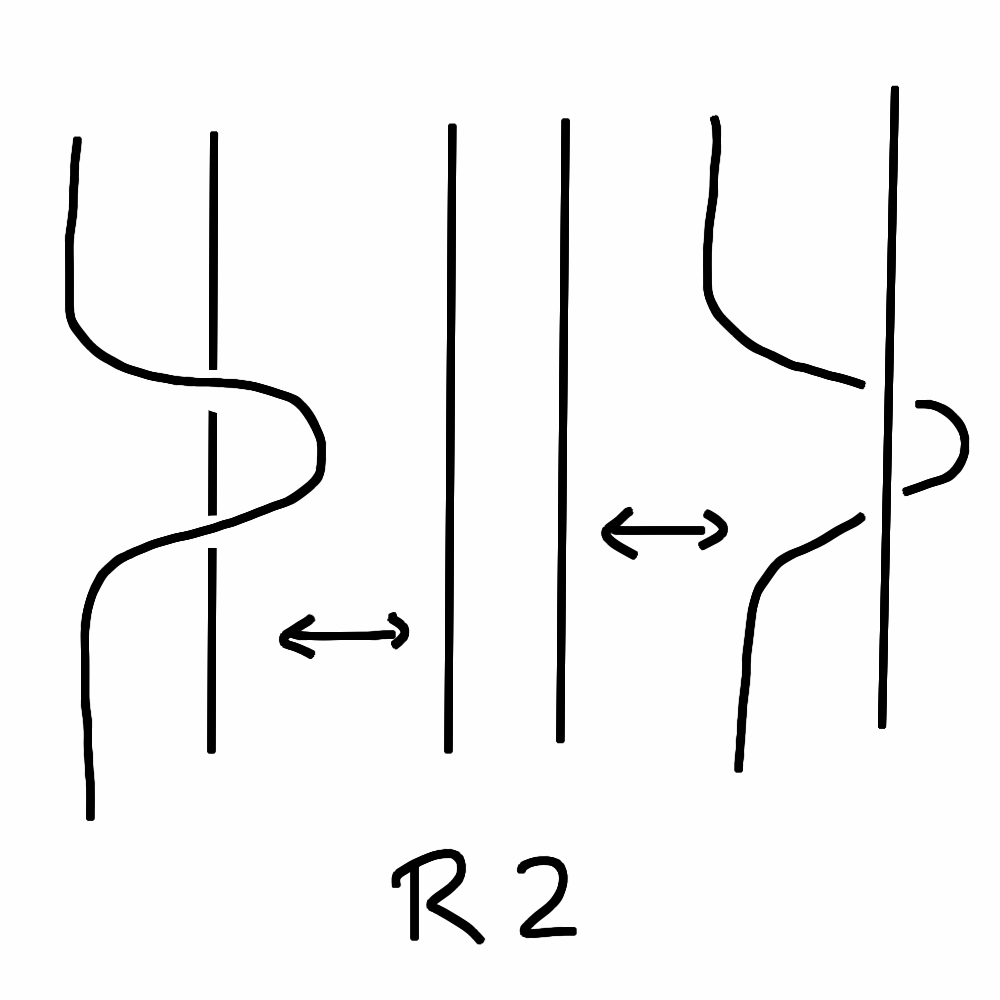
\includegraphics[width=.3\textwidth]{knotpics/r2.png}
    \caption{Type two Reidemeister moves.}
\end{figure}


\begin{exercise}
Explain why a type two Reidemeister move leaves tricolorability alone.
There are two possible colorings to deal with: either all of the strands have one single color, or all three colors are involved.
Be sure to check both of those, and moves in both directions.
\end{exercise}

For type three moves, I want you to work a bit more independently.

\begin{exercise}
Draw the possible pictures for colorings of type three Reidemeister moves, and use them to show that these moves preserve tricolorability of a knot or link.
\end{exercise}

\textbf{Attention:} This is a place where the Reidemeister moves redeem themselves.
There is no way to check ``every possible ambient isotopy'' and all of the resulting planar projections.
There are simply too many possible things one can do.
But there are only three types of Reidemeister moves.
That is way easier!
And thanks to Reidemeister we know that any ambient isotopy can be realized as a sequence of Reidemeister moves, so checking the moves is enough.

\subsection*{The Importance of Tricolorability}

We saw in the last reading that the unknot is not tricolorable, but the trefoil knot is tricolorable.
Now we have discussed why tricolorability is preserved by Reidemeister moves, and hence preserved by any ambient isotopy.

This means that there is no ambient isotopy between the unknot and the trefoil.
We have actually \emph{proved} that the trefoil knot and the unknot are not equivalent by ambient isotopy! They have different values of the tricolorability invariant (one ``yes'', one ``no''), so they must be different!


\begin{exercise}
Use the notion of tricolorability to show that this knot is different from the unknot.
\end{exercise}

\begin{figure}[h]
    \centering
    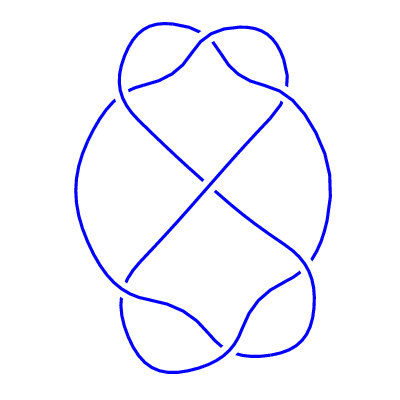
\includegraphics[width=.5\textwidth]{knotpics/7_4.png}
    \caption{A knot with seven crossings.}
\end{figure}

\begin{thebibliography}{9}

\bibitem{Adams}
	Colin C. Adams,
	\emph{The Knot Book},
	American Mathematical Society,
	2004.

\bibitem{knotinfo}
	J. C. Cha and C. Livingston,
	KnotInfo: Table of Knot Invariants,
	\url{http://www.indiana.edu/~knotinfo},
	accessed: September 6, 2013.


\end{thebibliography}

\end{document}
%sagemathcloud={"zoom_width":100}